\documentclass{beamer}
\usepackage{amsmath}
\usepackage{amsfonts}
\usepackage{mathtools}
\usepackage{enumerate}
\usepackage{biblatex}
\usepackage{tikz}
\usepackage{algorithm}
\usepackage{algorithmic}
\usepackage{hyperref}
\usepackage{graphicx}
\usepackage{listings}
\usepackage{xcolor}
\usepackage{subcaption}
\usepackage{forest}
\title{MATH 603 - Final Assignment}
\author{Aiden Taylor}
\institute{University of Calgary\\Department of Mathematics \& Statistics\\Calgary, AB, Canada}
\date{December 5th, 2024}

%\AtBeginSection[]
%{
%  \begin{frame}
%    \frametitle{Outline}
%    \tableofcontents[currentsection]
%  \end{frame}
%}

\AtBeginSubsection[]
{
  \begin{frame}
    \frametitle{Outline}
    \tableofcontents[currentsubsection]
  \end{frame}
}

\begin{document}
\frame{\titlepage}

\begin{frame}
\frametitle{The Problems}
	\begin{enumerate}[1.]
		\item Write a computer program to implement the Fast Fourier Transform (FFT).
	\item Using the FFT, write a computer program to solve numerically
		the initial-value problem (IVP) for the heat equation,
			\[
		\begin{cases}
			u_t = u_{xx} & (t,x) \in [0,T] \times [0,L] \\
			u(0,x) = u_0(x) & x \in [0,L]
		\end{cases}.
			\]
	\end{enumerate}
\end{frame}

\section{Problem 1}
\subsection{Discrete Fourier Transform}
\begin{frame}
	\frametitle{Continuous Fourier Transform}
	The Fourier Transform of some function $f(x)$ is given as
	\begin{equation*}
		F(\omega) = \hat{f}(\omega) = \mathcal{F}\left[f\right](\omega) = \frac{1}{2\pi}\int_{-\infty}^{\infty}{f(x)e^{-i\omega x}dx},
	\end{equation*}
	where the function can be recovered as
	\begin{equation*}
		f(x) = \int_{-\infty}^{\infty}{\hat{f}(\omega)e^{i\omega x}d\omega}.
	\end{equation*}
\end{frame}
\begin{frame}
	\frametitle{Discretization}
	Given $n \in \mathbb{N}$,
	\begin{equation*}
		\begin{cases}
			\omega_m = 2\pi m/n, & m = 0,1,\dots,n-1, \\
			x_k = x_0 + k\Delta x, & k = 0,1,\dots,n-1,
		\end{cases}
	\end{equation*}
	where $x_0 = 0$ and $\Delta x = L/(n-1)$.
\end{frame}
\begin{frame}
	\frametitle{DFT and IDFT}
	Letting $f_k = f(x_k)$, the DFT and Inverse DFT (IDFT) are given as
	\begin{equation*}
		f_{m}^{\#} = \sum_{k=0}^{n-1}{f_ke^{-i\omega_mk}}, \quad m = 0,1,\dots,n-1,
	\end{equation*}
	and
	\begin{equation*}
		f_{k} = \frac{1}{n}\sum_{m=0}^{n-1}{f_{m}^{\#}e^{i\omega_mk}}, \quad k = 0,1,\dots,n-1.
	\end{equation*}
\end{frame}
\begin{frame}
	Letting $\xi = e^{i2\pi/n}$, the DFT and IDFT can be written as
	\begin{equation*}
		\begin{bmatrix}
			f_{0}^{\#} \\
			f_{1}^{\#} \\
			f_{2}^{\#} \\
			\vdots \\
			f_{n-1}^{\#}
		\end{bmatrix}
		=
		\begin{bmatrix}
			1 & 1 & 1 & \dots & 1 \\
			1 & \xi^{-1} & \xi^{-2} & \dots & \xi^{-(n-1)} \\
			1 & \xi^{-2} & \xi^{-4} & \dots & \xi^{-2(n-1)} \\
			\vdots & \vdots & \vdots & \vdots & \vdots \\
			1 & \xi^{-(n-1)} & \xi^{-2(n-1)} & \dots & \xi^{-(n-1)(n-1)} 
		\end{bmatrix}
		\begin{bmatrix}
			f_{0} \\
			f_{1} \\
			f_{2} \\
			\vdots \\
			f_{n-1}
		\end{bmatrix},
	\end{equation*}
	\begin{equation*}
		\begin{bmatrix}
			f_{0} \\
			f_{1} \\
			f_{2} \\
			\vdots \\
			f_{n-1}
		\end{bmatrix}
		=
		\frac{1}{n}
		\begin{bmatrix}
			1 & 1 & 1 & \dots & 1 \\
			1 & \xi^{1} & \xi^{2} & \dots & \xi^{(n-1)} \\
			1 & \xi^{2} & \xi^{4} & \dots & \xi^{2(n-1)} \\
			\vdots & \vdots & \vdots & \vdots & \vdots \\
			1 & \xi^{(n-1)} & \xi^{2(n-1)} & \dots & \xi^{(n-1)(n-1)} 
		\end{bmatrix}
		\begin{bmatrix}
			f_{0}^{\#} \\
			f_{1}^{\#} \\
			f_{2}^{\#} \\
			\vdots \\
			f_{n-1}^{\#}
		\end{bmatrix},
	\end{equation*}
	where the computational complexity for each is $\mathcal{O}(n^2)$.
\end{frame}
\subsection{Fast Fourier Transform}
\begin{frame}
	\frametitle{Redundancies in the DFT}
	If $n=4$, then
	\begin{equation*}
		\begin{cases}
			f_{0}^{\#} &= f_0\xi^0 + f_1\xi^0 + f_2\xi^0 + f_3\xi^0 \\
			f_{1}^{\#} &= f_0\xi^0 + f_1\xi^{-1} + f_2\xi^{-2} + f_3\xi^{-3} \\
			f_{2}^{\#} &= f_0\xi^0 + f_1\xi^{-2} + f_2\xi^{-4} + f_3\xi^{-6} \\
			f_{3}^{\#} &= f_0\xi^0 + f_1\xi^{-3} + f_2\xi^{-6} + f_3\xi^{-9}.
		\end{cases}
	\end{equation*}
\end{frame}
\begin{frame}
	\frametitle{Redundancies in the DFT}
	Noticing that $\xi^0 = \xi^{-4} = 1$, $\xi^{-2} = \xi^{-6} = -1$, $\xi^{-1} = \xi^{-9} = -i$, and $\xi^{-3} = i$, then
\begin{equation*}
	\begin{cases}
		f_{0}^{\#} &= (f_0 + f_1) + \xi^0(f_2 + f_3) \\
		f_{1}^{\#} &= (f_0 - f_1) + \xi^{-1}(f_2 - f_3) \\
		f_{2}^{\#} &= (f_0 + f_1) + \xi^{-2}(f_2 + f_3) \\
		f_{3}^{\#} &= (f_0 - f_1) + \xi^{-3}(f_2 - f_3).
	\end{cases}
\end{equation*}
\end{frame}
\begin{frame}
	\frametitle{Cooley-Tukey Algorithm}
	If $n = 2^{\ell}$ where $\ell \in \mathbb{Z}^+$, then
	\begin{equation*}
		\begin{aligned}
			f_{m}^{\#} = \sum_{k=0}^{n-1}{f_k\xi^{-mk}} &= \sum_{k=0}^{\frac{n}{2}-1}{f_{2k}\xi^{-m(2k)}} + \sum_{k=0}^{\frac{n}{2}-1}{f_{2k + 1}\xi^{-m(2k+1)}} \\
			&= \sum_{k=0}^{\frac{n}{2}-1}{f_{2k}\xi^{-2mk}} + \xi^{-m}\sum_{k=0}^{\frac{n}{2}-1}{f_{2k + 1}\xi^{-2mk}},
		\end{aligned}
	\end{equation*}
	for $m = 0,1,\dots,n-1$.
\end{frame}
\begin{frame}
	\frametitle{Computation Complexity}
	The computational complexity of the Cooley-Tukey algorithm is $\mathcal{O}(n\log_2{n})$, which can be
	illustrated by the following binary tree,
	\begin{centering}
	\[
	\begin{tikzpicture}[level distance=1.00cm,
	  level 1/.style={sibling distance=6cm},
	  level 2/.style={sibling distance=3cm},
	  level 3/.style={sibling distance=1.5cm},
	  level 4/.style={sibling distance=0.75cm}]

	  \node {$cn$}
	    child {node {$cn/2$}
	      child {node {$cn/4$}
		child {node {$\vdots$}
		  child {node {$c$}}
		  child {node {$c$}}
		}
		child {node {$\vdots$}
		  child {node {$\ldots$}}
		  child {node {$\ldots$}}
		}
	      }
	      child {node {$cn/4$}
		child {node {$\vdots$}
		  child {node {$\ldots$}}
		  child {node {$\ldots$}}
		}
		child {node {$\vdots$}
		  child {node {$\ldots$}}
		  child {node {$\ldots$}}
		}
	      }
	    }
	    child {node {$cn/2$}
	      child {node {$cn/4$}
		child {node {$\vdots$}
		  child {node {$\ldots$}}
		  child {node {$\ldots$}}
		}
		child {node {$\vdots$}
		  child {node {$\ldots$}}
		  child {node {$\ldots$}}
		}
	      }
	      child {node {$cn/4$}
		child {node {$\vdots$}
		  child {node {$\ldots$}}
		  child {node {$\ldots$}}
		}
		child {node {$\vdots$}
		  child {node {$c$}}
		  child {node {$c$}}
		}
	      }
	    };
	\end{tikzpicture}
	\]
	\end{centering}
\end{frame}
\begin{frame}
	\frametitle{Height of the Binary Tree}
	At the bottom level we know that we should only need 
	\begin{equation*}
		cn/2^i = \mathcal{O}(1) = k
	\end{equation*}
	floating point operations for each node, and taking the logarithm of both sides gives us
	\begin{equation*}
		\begin{aligned}
			&\log_2{(cn/2^i)} = \log_2{k} \\
			&\Rightarrow\log_2{cn} - \log_2{2^i} = \log_2{k} \\
			&\Rightarrow\log_2{n} + \log_2{c} - i\log_2{2} = \log_2{k} \\
			&\Rightarrow\log_2{n} + \log_2{c} - \log_2{k} = i,
		\end{aligned}
	\end{equation*}
	which results in a height of $\mathcal{O}(\log_2{n})$ and an over all complexity of
	$\mathcal{O}(n\log_2{n})$.
\end{frame}
\begin{frame}
	\frametitle{The Algorithm}
	\includegraphics[scale=0.6]{fft_algorithm.png}
\end{frame}

\section{Problem 2}
\subsection{Solving Numerically}
\begin{frame}
	\frametitle{The IVP}
	Revisting Problem 2, our goal is to solve numerically the IVP,
			\[
		\begin{cases}
			u_t = u_{xx} & (t,x) \in [0,T] \times [0,L] \\
			u(0,x) = u_0(x) & x \in [0,L]
		\end{cases},
			\]
	using the FFT.
\end{frame}
\begin{frame}
	\frametitle{Fourier Transform of the Heat Equation}
	The Fourier Transform of $u$ and its derivatives are
	\begin{itemize}
		\item $u(t,x) \xRightarrow[]{\mathcal{F}} \hat{u}(t,\omega)$
		\item $u_t \xRightarrow[]{\mathcal{F}} \frac{d}{dt}\hat{u}(t,\omega)$
		\item $u_{xx} \xRightarrow[]{\mathcal{F}} -\omega^2\hat{u}(t,\omega)$
	\end{itemize}
	which gives us
	\begin{equation*}
		\frac{d}{dt}\hat{u}(t,\omega) = -\omega^2\hat{u}(t,\omega),
	\end{equation*}
	which has the solution
	\begin{equation*}
		\hat{u}(t,\omega) = \hat{u_0}e^{-\omega^2t}.
	\end{equation*}
\end{frame}
\begin{frame}
	\frametitle{Discretization}
	Given $n \in \mathbb{N}$,
	\begin{equation*}
		\begin{cases}
			\omega_m = 2\pi m/n, & m = 0,1,\dots,n-1, \\
			x_k = x_0 + k\Delta x, & k = 0,1,\dots,n-1,
		\end{cases}
	\end{equation*}
	where $x_0 = 0$ and $\Delta x = L/(n-1)$, then we have
	\begin{equation*}
		\begin{bmatrix}
			\frac{d}{dt}u^{\#}(t,\omega_0) \\
			\vdots \\
			\frac{d}{dt}u^{\#}(t,\omega_{n-1})
		\end{bmatrix}
		=
		\begin{bmatrix}
			-\omega_0^2u^{\#}(t,\omega_0) \\
			\vdots \\
			-\omega_{n-1}^2u^{\#}(t,\omega_{n-1})
		\end{bmatrix},
	\end{equation*}
	and
	\begin{equation*}
		\begin{bmatrix}
			u^{\#}(t,\omega_0) \\
			\vdots \\
			u^{\#}(t,\omega_{n-1})
		\end{bmatrix}
		=
		\begin{bmatrix}
			u_0^{\#}(t,\omega_0)e^{-\omega_0^2t} \\
			\vdots \\
			u_0^{\#}(t,\omega_{n-1})e^{-\omega_{n-1}^2t} \\
		\end{bmatrix}.
	\end{equation*}
\end{frame}
\subsection{Results}
\begin{frame}
	\frametitle{Example IVP}
	Consider,
			\[
			\begin{cases}
				u_t = u_{xx} & (t,x) \in [0,100] \times [0,1] \\
				u(0,x) = u_0(x) & x \in [0,1]
			\end{cases}
			\]
	where
	\begin{equation*}
		u_0 =
		\begin{cases}
			1 & x \in [0.3725,0.6235] \\
			0 & \text{otherwise}
		\end{cases}
	\end{equation*}
	and $n = 256$.
\end{frame}
\begin{frame}
	\frametitle{Initial-value Function}
	\begin{figure}[ht]
		\centering
		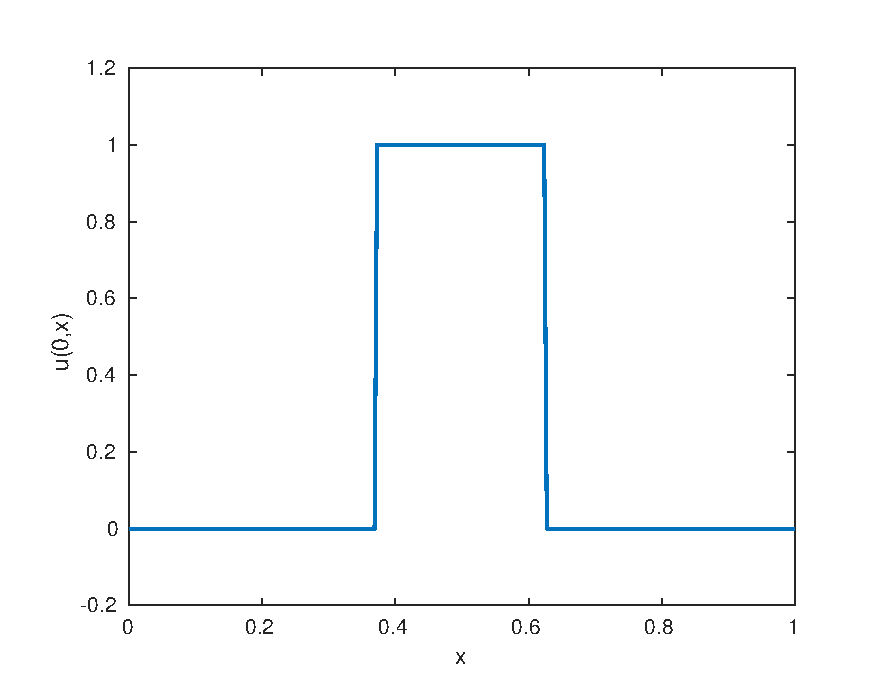
\includegraphics[scale=0.65]{../write-up/u0}
		\caption{Plot of $u_0(x)$.}
	\end{figure}
\end{frame}
\begin{frame}
	\frametitle{2-dimensional Plot}
	\begin{figure}[ht]
		\centering
		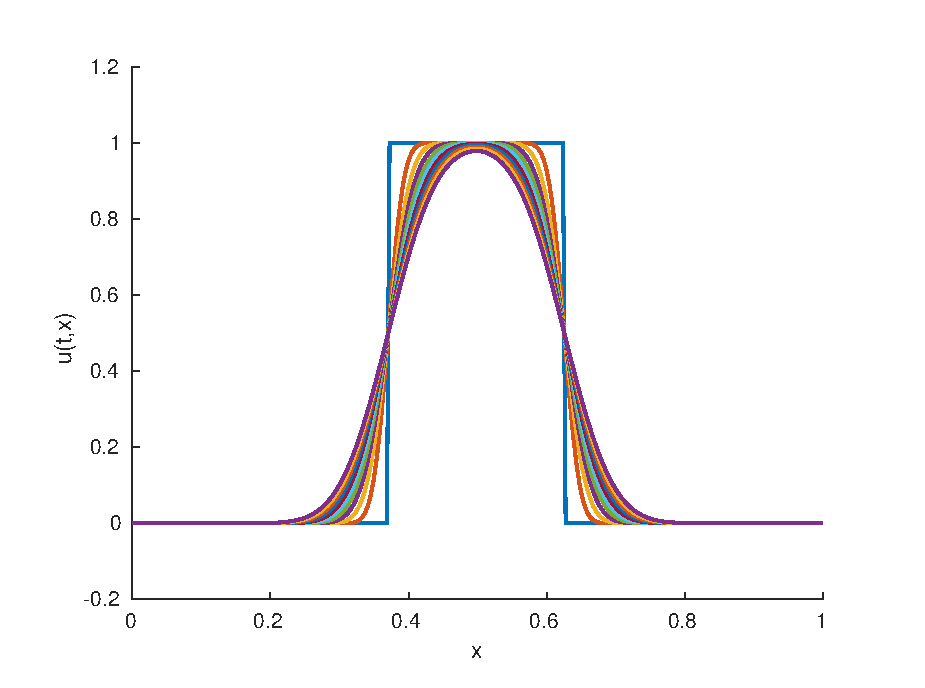
\includegraphics[scale=0.65]{../write-up/heat_eq_2d}
		\caption{2-dimensional plot of the numerical solution to the IVP.}
	\end{figure}
\end{frame}
\begin{frame}
	\frametitle{3-dimensional Plot}
	\begin{figure}[ht]
		\centering
		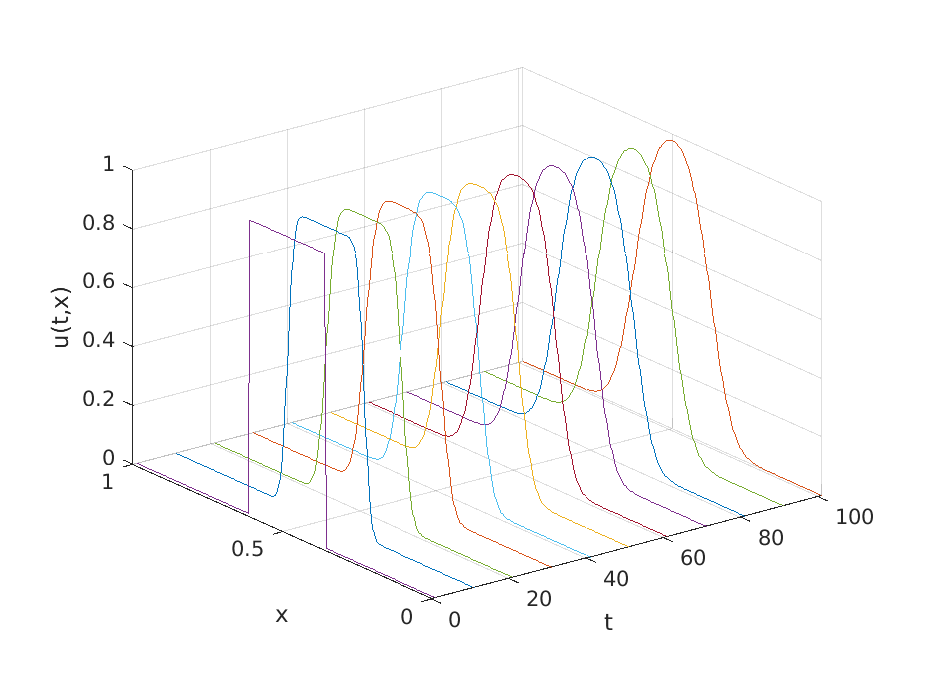
\includegraphics[scale=0.65]{../write-up/heat_eq_3d}
		\caption{3-dimensional plot of the numerical solution to the IVP.}
	\end{figure}
\end{frame}

\begin{frame}
	\begin{center}
		Thank you!
	\end{center}
\end{frame}
\end{document}
